\chapter{Analyse et Conception du Systeme :}

\section{Introduction}

Ce chapitre presente l'analyse fonctionnelle de l'application d'analyse de sentiments des commentaires d'Hespress destinee aux analystes, chercheurs et decideurs. L'objectif est de fournir une plateforme complete et performante pour la collecte automatisee, l'analyse et la visualisation des sentiments exprimes dans les commentaires du site d'actualites Hespress. Cette analyse detaillee etablira des directives pour le developpement d'une interface utilisateur intuitive et d'un systeme d'analyse robuste, mettant en avant les besoins d'analyse des donnees textuelles en temps reel.

L'application integre des technologies modernes comme Next.js pour le frontend, FastAPI pour le backend, Keycloak pour l'authentification, Selenium pour le web scraping, le modele cardiffnlp/twitter-xlm-roberta-base-sentiment pour la classification des sentiments, et Spring pour l'API Gateway. Un systeme convivial et performant servira de catalyseur pour une meilleure comprehension des opinions publiques et des tendances sociales.

\section{Identification des Besoins Utilisateurs}

Pour developper une application d'analyse de sentiments repondant aux besoins des utilisateurs, nous avons entrepris un processus approfondi d'etude de marche, incluant des analyses comportementales, des entretiens avec des experts en analyse de donnees et des sessions de definition des exigences avec les parties prenantes. Le besoin d'un acces simplifie aux donnees de sentiments, d'une plateforme flexible pour analyser les tendances d'opinion ainsi que d'outils de visualisation avances sont clairement apparus.

L'application doit faciliter une collecte automatisee des donnees, une analyse precise des sentiments et une presentation claire des resultats, tandis que les outils d'analyse doivent completer cette experience en fournissant des insights actionables sur les tendances d'opinion publique.

\begin{table}[H]
\centering
\begin{tabularx}{\textwidth}{|l|X|}
\hline
\textbf{Besoin identifie} & \textbf{Description du besoin} \\
\hline
Collecte automatisee des donnees & 
L'application doit offrir une interface permettant de configurer et de lancer automatiquement la collecte des commentaires d'Hespress via web scraping. \\
\hline
Analyse de sentiments en temps reel & 
Un systeme d'analyse utilisant des modeles de NLP avances pour classifier automatiquement les sentiments (positif, negatif, neutre) des commentaires collectes. \\
\hline
Visualisation et reporting & 
Des tableaux de bord interactifs et des rapports detailles pour visualiser les tendances de sentiments, generer des statistiques et suivre l'evolution des opinions dans le temps. \\
\hline
Gestion des utilisateurs et securite & 
Un systeme d'authentification robuste permettant la gestion des droits d'acces et la securisation des donnees sensibles. \\
\hline
\end{tabularx}
\caption{Besoins utilisateurs pour l'application d'analyse de sentiments}
\label{tab:besoins-utilisateurs}
\end{table}

En repondant a ces besoins, l'application d'analyse de sentiments represente un environnement d'analyse complet et integre, qui favorise la comprehension des opinions publiques et l'aide a la decision basee sur les donnees.

\section{Specification des Fonctionnalites}

La specification des fonctionnalites traduit les besoins utilisateurs en caracteristiques techniques et operationnelles concretes de l'application d'analyse de sentiments. Cette section detaille les fonctionnalites essentielles requises pour repondre aux exigences des analystes et des decideurs.

\begin{itemize}
    \item \textbf{Collecte de donnees} : Le module de collecte utilise \textbf{Selenium + FastAPI} pour assurer une collecte automatisee des commentaires d'Hespress. Cette fonctionnalite permet la configuration des parametres de scraping et la gestion des sessions, offrant ainsi une solution robuste pour l'acquisition continue de donnees textuelles.
    
    \item \textbf{Analyse de sentiments} : L'analyse est realisee grace au modele \textbf{cardiffnlp/twitter-xlm-roberta-base-sentiment}, qui assure une classification automatique des sentiments avec un support multilingue (arabe, français, darija) et un scoring de confiance pour chaque prediction.
    
    \item \textbf{Tableau de bord analytique} : Le frontend developpe avec \textbf{Next.js} offre une interface interactive permettant de visualiser les resultats d'analyse. Il integre des graphiques en temps reel et des filtres avances pour une exploration approfondie des donnees.
    
    \item \textbf{Gestion des utilisateurs} : \textbf{Keycloak} assure l'authentification securisee, la gestion des roles et le controle d'acces aux fonctionnalites selon les privileges des utilisateurs, garantissant ainsi la securite et la confidentialite des donnees.
    
    \item \textbf{API Gateway} : \textbf{Spring Gateway} centralise la gestion des requetes, assure le load balancing et securise les communications entre les differents microservices de l'architecture.
    
    \item \textbf{Stockage et historique} : La base de donnees permet la sauvegarde des donnees collectees et des resultats d'analyse, avec la possibilite d'effectuer des requetes historiques pour analyser l'evolution des sentiments dans le temps.
\end{itemize}

Ces fonctionnalites doivent etre developpees en tenant compte des meilleures pratiques de l'UX/UI pour assurer une facilite d'utilisation et engager activement les utilisateurs avec l'application d'analyse.

\section{Besoins non fonctionnels}

Pour completer les besoins fonctionnels, notre projet devra respecter quelques proprietes contribuant a une meilleure qualite de la solution obtenue. Parmi ces criteres, on retrouve :

\begin{itemize}
    \item \textbf{Performance} : Il s'agit d'optimiser le temps de traitement des donnees textuelles ainsi que d'utiliser les bonnes pratiques du developpement. L'analyse de sentiments doit etre rapide et efficace meme avec de gros volumes de donnees.
    
    \item \textbf{Evolutivite} : L'application doit pouvoir integrer de nouveaux modeles d'analyse, de nouvelles sources de donnees ou de nouvelles fonctionnalites sans modifier les modules deja existants.
    
    \item \textbf{Securite} : L'acces a l'application et aux donnees doit etre securise. Pour gerer les autorisations aux differents modules de l'application, nous utilisons Keycloak pour l'authentification et Spring Gateway pour la securisation des APIs.
    
    \item \textbf{Haute disponibilite} : L'application doit etre disponible en permanence, minimisant les temps d'arret et assurant un fonctionnement continu meme en cas de defaillance d'une partie du systeme.
    
    \item \textbf{Scalabilite} : Le systeme doit pouvoir gerer une augmentation du volume de donnees a analyser et du nombre d'utilisateurs simultanement connectes.
    
    \item \textbf{Precision d'analyse} : Les resultats d'analyse de sentiments doivent etre fiables et precis, avec un taux d'erreur minimal pour garantir la qualite des insights generes.
\end{itemize}

\section{Fonctionnalites attendues}

Les cas d'utilisation detailles illustrent les interactions typiques entre les utilisateurs et l'application d'analyse de sentiments. Ils permettent de visualiser les scenarios quotidiens et d'identifier les points de contact entre l'utilisateur et le systeme.

\subsection{Configuration de la collecte de donnees}

\textbf{Acteurs} : Administrateur, Analyste

\textbf{Prerequis} : L'utilisateur est connecte a son compte et possede les droits necessaires.

\textbf{Scenario principal} :
\begin{enumerate}
    \item L'utilisateur selectionne l'option 'Configuration de Collecte' dans le menu.
    \item Il definit les parametres de scraping (frequence, mots-cles, sections cibles).
    \item Il configure les filtres de collecte et valide les parametres.
    \item L'utilisateur lance la collecte automatisee en cliquant sur 'Demarrer la collecte'.
    \item Le systeme enregistre la configuration et demarre le processus de collecte.
\end{enumerate}

\subsection{Analyse de sentiments en temps reel}

\textbf{Acteurs} : Analyste, Chercheur

\textbf{Prerequis} : Des donnees sont disponibles dans le systeme.

\textbf{Scenario principal} :
\begin{enumerate}
    \item L'utilisateur selectionne l'option 'Analyse de Sentiments' dans le menu.
    \item Il choisit la periode d'analyse et les filtres souhaites.
    \item Il lance l'analyse en cliquant sur 'Analyser les sentiments'.
    \item Le systeme traite les donnees avec le modele XLM-RoBERTa.
    \item Les resultats sont affiches avec des visualisations interactives.
\end{enumerate}

\subsection{Consultation du tableau de bord analytique}

\textbf{Acteurs} : Decideur, Analyste, Chercheur

\textbf{Prerequis} : L'utilisateur est connecte a son compte.

\textbf{Scenario principal} :
\begin{enumerate}
    \item L'utilisateur accede au tableau de bord principal.
    \item Il consulte les metriques en temps reel et les tendances.
    \item Il utilise les filtres pour affiner les donnees affichees.
    \item L'utilisateur genere des rapports personnalises selon ses besoins.
    \item Il exporte les resultats dans differents formats (PDF, Excel, CSV).
\end{enumerate}

\subsection{Gestion des utilisateurs par l'administrateur}

\textbf{Acteurs} : Administrateur

\textbf{Prerequis} : L'administrateur est connecte a son compte administrateur.

\textbf{Scenario principal} :
\begin{enumerate}
    \item L'administrateur selectionne l'option 'Gestion des Utilisateurs' dans Keycloak.
    \item Il consulte la liste des utilisateurs inscrits sur la plateforme.
    \item L'administrateur ajoute, supprime ou modifie les roles et permissions.
    \item Il configure les politiques d'acces selon les besoins de securite.
    \item Le systeme enregistre les modifications et met a jour les autorisations.
\end{enumerate}

\subsection{Monitoring et maintenance du systeme}

\textbf{Acteurs} : Administrateur technique

\textbf{Prerequis} : L'administrateur a acces aux outils de monitoring.

\textbf{Scenario principal} :
\begin{enumerate}
    \item L'administrateur accede au tableau de bord de monitoring.
    \item Il verifie les performances des differents composants du systeme.
    \item Il consulte les logs d'erreur et les metriques de performance.
    \item L'administrateur effectue les maintenances preventives necessaires.
    \item Il configure les alertes pour le monitoring proactif.
\end{enumerate}

Ces cas d'utilisation representent des interactions frequentes et essentielles qui doivent etre prises en compte pour une experience utilisateur coherente et satisfaisante dans le contexte de l'analyse de sentiments.

\section{Backlog Produit}

Le developpement de notre application d'analyse de sentiments s'est structure autour d'un backlog produit bien defini, comprenant plusieurs epopees et user stories. Chaque user story a ete accompagnee de criteres d'acceptation clairs pour garantir la qualite et la conformite aux attentes.

\subsection{Epopee 1 : Infrastructure et Configuration}

\textbf{User Story 1.1 : Configuration de l'environnement de developpement}
\begin{itemize}
    \item En tant que developpeur
    \item Je veux configurer l'environnement avec Next.js, FastAPI, Keycloak et Spring Gateway
    \item Afin de disposer d'une base technique solide
    \item \textbf{Criteres d'acceptation :}
    \begin{itemize}
        \item Tous les services sont deployes et communicants
        \item L'authentification Keycloak fonctionne correctement
        \item L'API Gateway route les requetes appropriees
    \end{itemize}
\end{itemize}

\textbf{User Story 1.2 : Integration du modele d'analyse de sentiments}
\begin{itemize}
    \item En tant que developpeur
    \item Je veux integrer le modele cardiffnlp/twitter-xlm-roberta-base-sentiment
    \item Afin de pouvoir analyser les sentiments des textes
    \item \textbf{Criteres d'acceptation :}
    \begin{itemize}
        \item Le modele est charge et operationnel
        \item L'API d'analyse retourne des predictions precises
        \item Le support multilingue (arabe, français) fonctionne
    \end{itemize}
\end{itemize}

\subsection{Epopee 2 : Collecte et Traitement des Donnees}

\textbf{User Story 2.1 : Developpement du module de web scraping}
\begin{itemize}
    \item En tant qu'analyste
    \item Je veux collecter automatiquement les commentaires d'Hespress
    \item Afin d'avoir des donnees fraiches pour l'analyse
    \item \textbf{Criteres d'acceptation :}
    \begin{itemize}
        \item Selenium collecte les commentaires sans erreur
        \item Les donnees sont structurees et stockees correctement
        \item Le processus est configurable et planifiable
    \end{itemize}
\end{itemize}

\textbf{User Story 2.2 : Preprocessing et nettoyage des donnees}
\begin{itemize}
    \item En tant que systeme
    \item Je veux nettoyer et preprocesser les textes collectes
    \item Afin d'ameliorer la qualite de l'analyse
    \item \textbf{Criteres d'acceptation :}
    \begin{itemize}
        \item Les textes sont normalises et nettoyes
        \item Les caracteres speciaux et spam sont filtres
        \item Les donnees sont prete pour l'analyse
    \end{itemize}
\end{itemize}

\subsection{Epopee 3 : Interface Utilisateur et Visualisation}

\textbf{User Story 3.1 : Developpement du tableau de bord}
\begin{itemize}
    \item En tant qu'analyste
    \item Je veux visualiser les resultats d'analyse sur un tableau de bord interactif
    \item Afin de comprendre les tendances de sentiments
    \item \textbf{Criteres d'acceptation :}
    \begin{itemize}
        \item Le tableau de bord affiche les metriques en temps reel
        \item Les graphiques sont interactifs et informatifs
        \item Les filtres permettent d'affiner les donnees
    \end{itemize}
\end{itemize}

\textbf{User Story 3.2 : Generation de rapports}
\begin{itemize}
    \item En tant que decideur
    \item Je veux generer des rapports detailles sur les analyses
    \item Afin de prendre des decisions informees
    \item \textbf{Criteres d'acceptation :}
    \begin{itemize}
        \item Les rapports sont generes automatiquement
        \item Plusieurs formats d'export sont supportes
        \item Les donnees sont precises et a jour
    \end{itemize}
\end{itemize}

\subsection{Sprint Plan}

\textbf{Sprint 1} : Configuration de l'environnement (User Story 1.1), Integration du modele d'analyse (User Story 1.2)

\textbf{Sprint 2} : Developpement du web scraping (User Story 2.1), Preprocessing des donnees (User Story 2.2)

\textbf{Sprint 3} : Developpement du tableau de bord (User Story 3.1), Interface d'authentification

\textbf{Sprint 4} : Generation de rapports (User Story 3.2), Optimisation et deploiement

\section{PLANIFICATION DU PROJET}

Le diagramme de Gantt suivant presente le planning du projet, indiquant les differentes phases de developpement et les delais associes pour l'application d'analyse de sentiments.

\subsection{PLANNING PREVISIONNEL}

\begin{figure}[H]
\centering
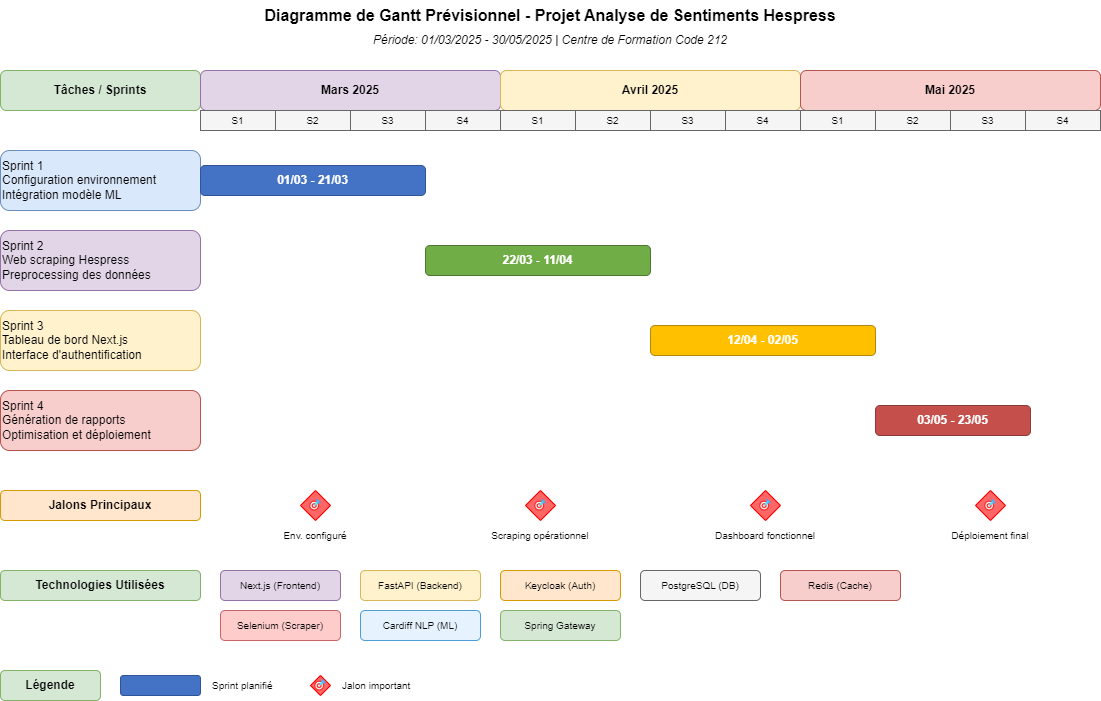
\includegraphics[height=8cm , width=\textwidth]{assets/images/gantt-previsionnel.png}
\caption{Diagramme de Gantt previsionnel pour le projet d'analyse de sentiments}
\label{fig:gantt-prev}
\end{figure}

\subsection{PLANNING REEL}

\begin{figure}[H]
\centering
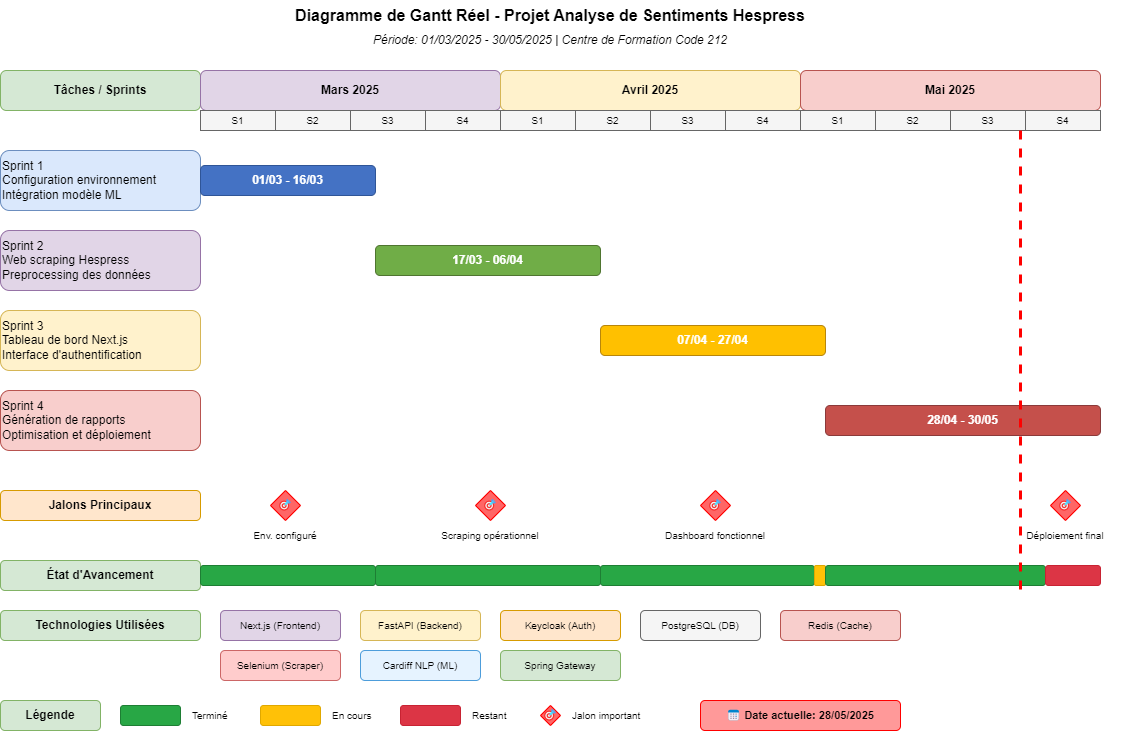
\includegraphics[height=8cm , width=\textwidth]{assets/images/gantt-reel.png}
\caption{Diagramme de Gantt reel pour le projet d'analyse de sentiments}
\label{fig:gantt-reel}
\end{figure}

\section{Diagramme de Cas d'Utilisation globale}

Le diagramme de cas d'utilisation offre une representation graphique des fonctionnalites du systeme d'analyse de sentiments telles qu'elles sont experimentees par les differents acteurs. Il identifie les interactions entre les utilisateurs (analyste, administrateur, decideur) et le systeme et illustre les principaux scenarios d'utilisation.

\begin{figure}[H]
\centering
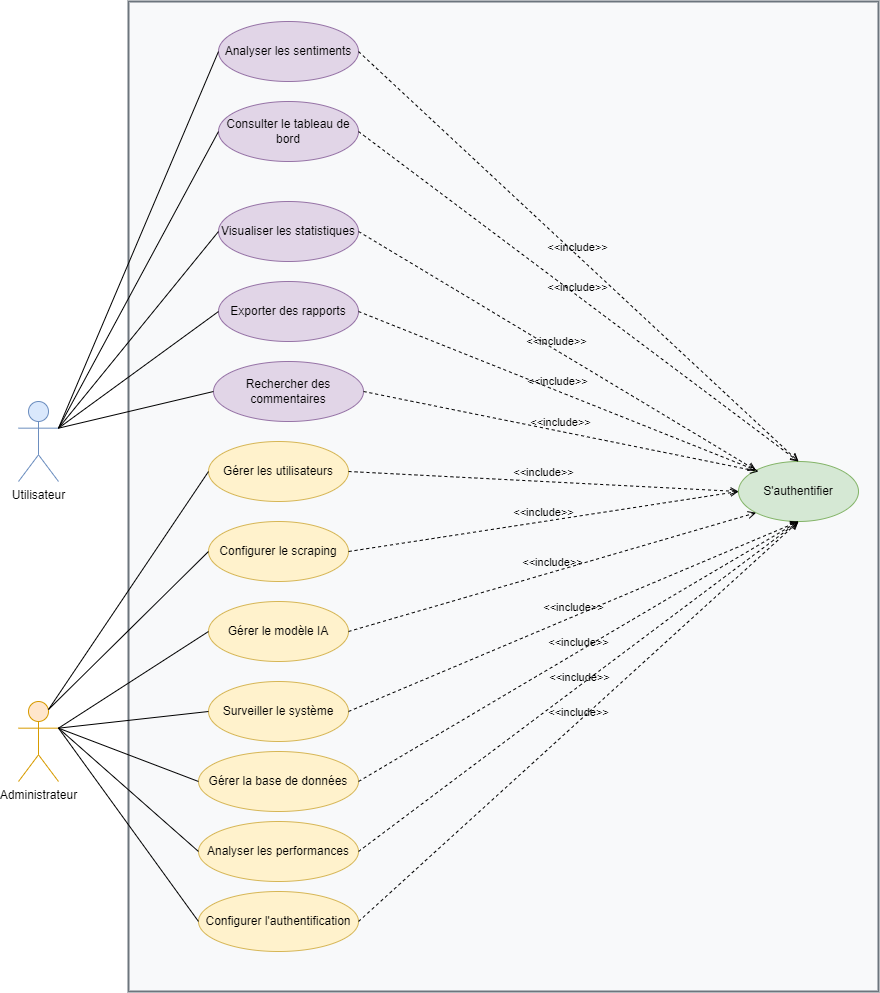
\includegraphics[height=20cm , width=\textwidth]{assets/images/usecase.png}
\caption{Diagramme de cas d'utilisation pour l'application d'analyse de sentiments}
\label{fig:usecase-global}
\end{figure}

\section{Diagramme de Classes globale}

Le diagramme de classes est essentiel pour visualiser la structure statique de l'application d'analyse de sentiments et decrire les objets encapsules dans le systeme ainsi que leurs relations. Il fournit une vue d'ensemble des classes, de leurs attributs, methodes et des associations inter-classes qui modelisent les donnees de l'application.

\begin{figure}[H]
\centering
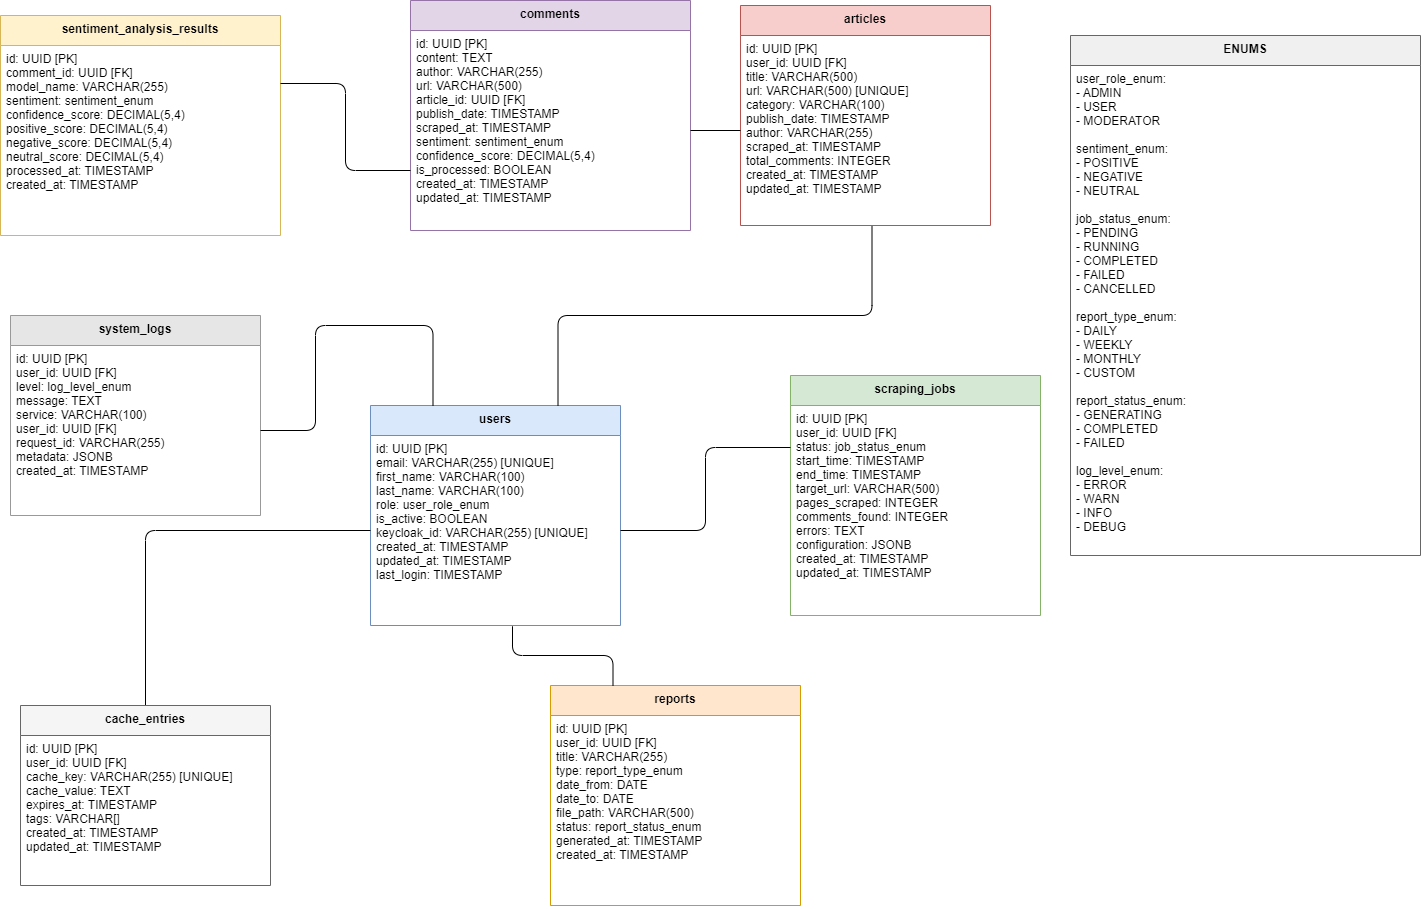
\includegraphics[height=12cm , width=\textwidth]{assets/images/class.png}
\caption{Diagramme de classes pour l'application d'analyse de sentiments}
\label{fig:class-global}
\end{figure}

\section{Architecture du Systeme}

L'architecture de l'application d'analyse de sentiments suit une approche microservices moderne, integrant les technologies specifiees pour assurer performance, scalabilite et maintenabilite.


\subsection{Composants de l'architecture}

\begin{itemize}
    \item \textbf{Frontend (Next.js)} : Interface utilisateur reactive et moderne
    \item \textbf{API Gateway (Spring)} : Point d'entree unique pour toutes les requetes
    \item \textbf{Service d'authentification (Keycloak)} : Gestion securisee des utilisateurs
    \item \textbf{Service de collecte (Selenium + FastAPI)} : Web scraping automatise
    \item \textbf{Service d'analyse (FastAPI + XLM-RoBERTa)} : Traitement et analyse des sentiments
    \item \textbf{Base de donnees} : Stockage des donnees collectees et des resultats
\end{itemize}

\section{Conclusion de Conception}

La conception de l'application d'analyse de sentiments suppose la creation d'une architecture robuste et evolutive qui repond aux besoins fonctionnels tout en offrant une experience utilisateur transparente et performante. Les diagrammes et modeles presentes dans ce chapitre constituent le socle pour les developpements futurs et pour l'implementation du systeme.

L'integration des technologies modernes (Next.js, FastAPI, Keycloak, Spring Gateway) avec des modeles d'IA avances (XLM-RoBERTa) permet de creer une solution complete pour l'analyse automatisee des sentiments dans les commentaires d'Hespress. Cette approche garantit une analyse precise, scalable et securisee des opinions publiques exprimees en ligne.

